% =============================================================================
% CS224R Final Report Template
% =============================================================================
% This template is structured for your CS224R final report with two main parts:
%   1. One-page extended abstract (required as first page)
%   2. Main paper (recommended ~8 pages)
%
% The extended abstract summarizes your project's main findings and accomplishments.
% The main paper details your methods, prior work, contributions, and results.
%
% For project groups, include a breakdown of individual contributions.
% =============================================================================

\documentclass{article}

\usepackage[preprint]{cs224r_2026}
\usepackage[utf8]{inputenc} % allow utf-8 input
\usepackage[T1]{fontenc}    % use 8-bit T1 fonts
\usepackage{hyperref}       % hyperlinks
\usepackage{url}            % simple URL typesetting
\usepackage{booktabs}       % professional-quality tables
\usepackage{amsfonts}       % blackboard math symbols
\usepackage{nicefrac}       % compact symbols for 1/2, etc.
\usepackage{microtype}      % microtypography
\usepackage{xcolor}         % colors
\usepackage{amsmath}
\usepackage{graphicx}       % for including figures
\usepackage{lipsum}         % for placeholder text

\title{Learning Priority Functions for Graph-Based Exploration in ARC-AGI-3}

\author{%
  Ryan Bookman \\
  Department of Computer Science\\
  Stanford University\\
  \texttt{rbookman@stanford.edu} \\
  % examples of more authors
  \And
  Steve Mendeleev \\
  Department of Computer Science\\
  Stanford University\\
  \texttt{steveroy@stanford.edu} \\
  \And
  Kyle Feinstein \\
  Department of Computer Science\\
  Stanford University\\
  \texttt{kfeinst@stanford.edu} \\
}

\begin{document}

% ============================================================================
% PART 1: ONE-PAGE EXTENDED ABSTRACT
% ============================================================================
\begin{titlepage}
\begin{center}
\Large\textbf{Extended Abstract}
\end{center}
\vspace{10pt}


\paragraph{Motivation} ARC-AGI-3 is an interactive benchmark where agents must discover unknown game mechanics through exploration under a strict action budget. One of the current state-of-the-art training-free approaches (Rudakov et al., 2025) tracks visited states in a directed graph and uses a hand-coded heuristic to assign each visual segment to one of five priority groups, which determines which parts of the screen to click first. This heuristic cannot adapt: a segment type that proves useless in level 1 receives the same priority in level 8. We ask whether replacing this fixed priority function with a learned one improves exploration efficiency across the progressively harder levels of ARC-AGI-3.

\paragraph{Method} We implement five learned priority agents on top of the Rudakov et al. graph explorer, all trained online from a dense $\pm 1$ binary reward signal (whether clicking a segment caused a visual state transition). Each agent ranks segments into five priority groups using a learned scoring function; the graph explorer's traversal logic is otherwise untouched. We also redesign the feature representation for each segment, replacing the three binary features of the original paper with four features, three of which are continuous, that better allow the model to discover gradients within categories. Additionally, all learned agents are warm-started from a weight configuration calibrated to approximately recover the heuristic's priority ordering.

\paragraph{Implementation} The five agents span a range of online learning approaches: (1) REINFORCE (vanilla policy gradient) for simplicity and interpretability; (2) First-Order MAML (FOMAML), which meta-learns an initialization that adapts quickly at level boundaries, exploiting the fact that different levels reward different segment types; (3) a two-layer MLP trained by online backpropagation as a nonlinear supervised baseline; (4) Soft Actor-Critic (SAC), for off-policy sample efficiency via a replay buffer with twin critics and entropy regularization; and (5) Proximal Policy Optimization (PPO), for stable on-policy updates with a clipped surrogate objective and GAE-$\lambda$ advantage estimates.

\paragraph{Results} In 45-minute evaluations on ARC-AGI's vc33 clicking game, FOMAML achieves a score of 4.42 vs. the baseline's 0.59, a 7.5× improvement, while REINFORCE reaches 2.82 and SAC 2.41. PPO (0.54) and the neural network (0.04) underperform the baseline in this time window, which we attribute to insufficient data for their respective sample requirements.

\paragraph{Discussion} The dominance of FOMAML confirms that the primary bottleneck is fast per-level adaptation rather than globally-optimal policy quality. Different levels introduce distinct interactive elements, so an initialization trained for quick adaptation consistently outperforms a single accumulated weight vector. The gap between REINFORCE and the baseline validates the core hypothesis that soft continuous weights over a richer feature space improve on fixed binary rules even with the simplest gradient update. The underperformance of PPO and the MLP illustrates that models with more parameters and richer objectives require more data before they outperform a warm-started linear baseline, and online RL in sparse environments can push these models toward bad local optima if they cannot accumulate enough signal early.

\paragraph{Conclusion} Replacing a hand-coded priority heuristic with a learned priority function, particularly one that meta-learns across levels, substantially improves exploration efficiency in ARC-AGI-3. The result suggests that the level-to-level distribution shift in ARC-AGI-3 is the dominant challenge, and that fast adaptation mechanisms are better matched to this environment than globally-optimized policies trained over the full game. 

\end{titlepage}

% ============================================================================
% PART 2: MAIN PAPER
% ============================================================================
\maketitle

\begin{abstract}
We extend the state-of-the-art graph-based exploration approach for ARC-AGI-3 (Rudakov et al., 2025) by replacing its hand-coded visual salience heuristic with five learned priority functions trained online from a dense binary transition reward. The heuristic assigns each visual segment to one of five priority groups using fixed binary rules that cannot adapt as levels progress. We redesign the segment feature representation from three binary indicators to four continuous features: HSV color saturation, a Gaussian closeness-to-medium-size score, status-bar membership, and a log-count of twin segments. We warm-start all learned agents to approximately recover the heuristic's ordering before any training begins. We compare five algorithms: REINFORCE, First-Order MAML (FOMAML), a two-layer MLP, Soft Actor-Critic (SAC), and Proximal Policy Optimization (PPO). In 45-minute evaluations on vc33, FOMAML achieves a 7.5x improvement in score over the baseline, REINFORCE achieves a 4.8x improvement, and SAC achieves a 4.1x improvement. PPO and the MLP underperform the baseline in this time window due to insufficient data for their sample requirements. These results establish that fast per-level meta-adaptation is the most effective inductive bias for this environment, and that learned continuous feature representations outperform hard-coded binary ones even with simple linear models.
\end{abstract}

\section{Introduction}
ARC-AGI-3 (ARC Prize Foundation 2025) represents a fundamental departure from prior ARC benchmarks. It presents game-like interactive environments where agents must discover unknown mechanics through exploration, forming hypotheses about what to click, testing them, and revising their understanding as levels progressively introduce new unknown elements. The benchmark penalizes both failure to solve levels and inefficiency in doing so, creating strong pressure for agents that find the right actions quickly.

Rudakov et al. (2025) establish a strong training-free baseline through systematic graph-based exploration. Their agent maintains a directed graph over visited states and action transitions, prioritizes actions using three binary visual salience features, and navigates toward unexplored frontier states using shortest-path distances. This structured approach substantially outperforms both random exploration and LLM-based baselines. However, the method is entirely static. Within each priority group, action selection is uniform at random, and the priority group assignments are determined by a heuristic that never updates. This means the agent wastes identical effort re-testing segment types that proved useless in level 1 when it encounters them again in level 8.

Our contribution is replacing this fixed priority function with a family of learned alternatives, while keeping the graph explorer's traversal logic entirely intact. Our hypothesis is that priority group assignment can be framed as an online supervised learning problem with a dense reward signal. For each segment clicked, the agent immediately observes whether that click caused a state transition (+1) or not (-1). This allows us to train policies using a per-click signal that is much more dense than the environment's extremely sparse level-completion reward.

We make three concrete contributions. First, we redesign the segment feature representation by replacing three binary indicators with four continuous features that preserve the heuristic's intended structure while permitting soft gradients. Second, we warm-start all learned agents to approximately recover the heuristic's priority ordering, ensuring competent behavior from the first step. Third, we implement and compare five online learning algorithms spanning policy gradient, meta-learning, supervised MLP, off-policy actor-critic, and on-policy clipped surrogate methods.

\begin{figure}[h]
  \centering
  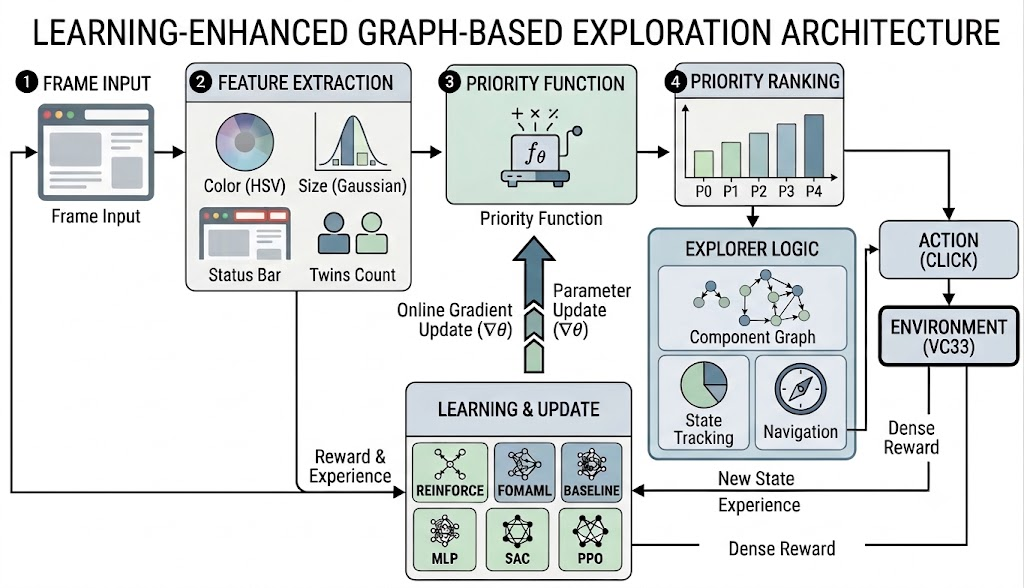
\includegraphics[width=0.95\linewidth]{SummaryDiagram.png}
  \caption{Visualization of our methods.}
  \label{fig:quantitative_results}
\end{figure}

Our main finding is that FOMAML, which meta-learns an initialization from which per-level weights can adapt quickly, achieves the largest gains, followed by vanilla REINFORCE and SAC. This pattern reveals that the dominant challenge in ARC-AGI-3 is not learning a globally optimal priority function across all levels, but adapting quickly to the specific interactive elements each level introduces.

\section{Related Work}

ARC-AGI-3~\cite{arcagi3} is a benchmark designed to measure general fluid intelligence, emphasizing adaptability to novel tasks. Agents are placed in unfamiliar turn-based games with no instructions and must discover the rules through interaction, under a strict action budget. Crucially, the scoring rewards not just solving levels but solving them efficiently, which makes the order in which an agent tests actions a first-order determinant of performance.

The most directly relevant prior work is Rudakov et al.~\cite{rudakov2025graph}, one of the strongest ARC-AGI-3 submissions, which serves as the baseline we build on. Their training-free agent maintains a directed graph of visited states and tested transitions, navigating toward unexplored frontiers via shortest paths. To make the large action space tractable, it ranks segments into five priority tiers using a fixed hand-coded heuristic over color, size, and morphology. This graph-based structure is motivated by Go-Explore~\cite{ecoffet2021first}, which shows that explicitly tracking visited states and reliably returning to frontier states outperforms memoryless search under sparse feedback. We keep this structure entirely intact and replace only the fixed priority heuristic with learned alternatives.

The core challenge is that ARC-AGI-3 levels shift over time, introducing new interactive elements as the agent progresses, so a fixed priority rule that works early on becomes stale. This motivates replacing the heuristic with a learned priority function trained online from per-click transition feedback. Alet et al.~\cite{alet2020metalearning} show that exploration strategies can be meta-learned across tasks so the agent adapts quickly when the environment changes, rather than relying on a fixed hand-designed bonus. SIERL~\cite{sierl2026} demonstrates more concretely that learning which frontier states to prioritize outperforms fixed heuristics in sparse-reward exploration. Neither work is applied to ARC-AGI-3, but both motivate the approach we take. We evaluate a range of online learning algorithms as priority-function learners, from simple policy gradient methods to off-policy actor-critic approaches, with FOMAML as the conceptual center given the level-shifting structure of the benchmark.

\section{Method}
\subsection{Baseline: Heuristic Priority Assignment}

The Rudakov et al. baseline computes three binary features per visual segment and uses hard-coded thresholds to assign each segment to one of five priority tiers:

\begin{table}[h]
\centering
\caption{Baseline Heuristic Feature Rules}
\label{tab:baseline_features}
\begin{tabular}{ll}
\toprule
\textbf{Feature} & \textbf{Rule} \\
\midrule
\texttt{is\_salient} & 1 if the color is white, gray, or black; else 0 \\
\texttt{is\_medium\_width} & 1 if bounding box spans 2--32 px in both $x$ and $y$; else 0 \\
\texttt{is\_status\_bar} & 1 if color index represents the masked status bar element; else 0 \\
\bottomrule
\end{tabular}
\end{table}

Segments with $\texttt{is\_status\_bar} = 1$ are assigned to the lowest priority group. Among the remaining segments, those matching both $\texttt{is\_salient}$ and $\texttt{is\_medium\_width}$ receive the highest priority. These rule encode the authors' intuitions that medium-sized, colorful elements are the most likely to be interactive buttons. However, crucially, this priority assignment remains identical at every step of every level and cannot adapt in response to agent experience.

\subsection{Problem Reformulation: Learning Priority Functions}

We reframe priority assignment as an online supervised learning problem. At each step, the agent selects a visual segment based on its current priority function, executes a click action, and immediately observes a dense binary reward: $r = +1$ if the frame transitioned to a new state, and $r = -1$ otherwise. This per-click signal allows online gradient updates after every single action, avoiding the extremely sparse level-completion signal that traditional end-to-end reinforcement learning approaches face with these games.

All five of our learned agents share a common architectural backbone. A parameterized scoring function $f_\theta(\phi)$ maps a segment's 4-dimensional feature vector $\phi$ to a scalar score. Visual segments are ranked by this score and partitioned evenly into five priority groups. The downstream graph explorer then selects from the highest available priority group using its existing navigation logic (the same navigation logic that Rudakov et al. presents). We update the parameters $\theta$ online after each clicked segment using the observed binary reward. 

Our design leaves the graph explorer's traversal strategy and state tracking completely unchanged, ensuring that any performance gains are isolated and directly attributable to priority learning.

\subsection{Feature Engineering}

We replace the three binary features of the baseline with four features, three of which are continuous. The motivation for this shift is twofold. First, binary features discard critical within-category information: all chromatic colors are treated identically by $\texttt{is\_salient}$, yet a highly saturated red segment and a muted pale-green segment carry vastly different interactive probabilities. Second, linear models over binary features can only express strict threshold decisions, whereas continuous features allow gradients to express graded preferences.

\textbf{Feature 1: HSV Color Saturation} (replaces \texttt{is\_salient}). We compute saturation directly from the RGB values:
\begin{equation}
\text{sat} = \frac{\max(R,G,B) - \min(R,G,B)}{\max(R,G,B)}
\end{equation}
While the original binary feature treats all chromatic colors identically, saturation preserves the salient/non-salient distinction while exposing a continuous gradient within the chromatic range. This, in contrast with a one-hot vector representing color, allows a model to learn that highly saturated game elements are more likely to be interactive than muted chromatic background elements.

\textbf{Feature 2: Closeness-to-Medium} (replaces \texttt{is\_medium\_width}). The binary $\texttt{is\_medium\_width}$ feature treats segment size as a hard classification (either medium or not), discarding all information about how far a segment deviates from the ideal scale. A continuous alternative like log(area) partially addresses this but can only encode a monotone preference ("bigger is better" or "smaller is better"), failing to capture the inverted-U shape the heuristic intends. Instead, we want a score that peaks at the ideal medium size and decays gracefully as segments grow too small or too large. We therefore compute a Gaussian response in log-area space:
\begin{equation}
\text{closeness} = \exp\left(-\frac{|\log(1 + \text{area}) - \log(1 + 64)|}{2.5}\right)
\end{equation}
This yields a score of 1.0 at the ideal scale and decreases smoothly toward 0 for segments 
that deviate in either direction,so a segment \textit{near} the medium range still receives 
a high score, while one far outside it scores near zero. The center at area $= 64\ \text{px}^2$ 
is the geometric mean of the 2--32 px medium range in each dimension: 
$(\sqrt{2 \times 32})^2 = 64$. We chose the bandwidth parameter $\sigma = 2.5$ so the half-response point falls exactly at the boundaries of the medium range.

\textbf{Feature 3: \texttt{is\_status\_bar}} (unchanged). Status-bar membership remains binary and the existing rule-based detection is highly reliable, meaning a continuous extension is not necessary.

\textbf{Feature 4: $\log(1 + \text{number\_of\_twins})$} (new feature). Segments with many twins (other segments sharing the identical area, rectangularity, and color) tend to represent repeating UI decoration patterns, such as life-dot indicators or score grids, rather than unique interactive objects. We apply a log transform rather than passing the raw count because the structural distinction between 0 and 1 twins (unique vs. non-unique) is far more informative than the distinction between 10 and 11 twins, and the log scaling keeps the feature magnitude inline with the others to prevent gradient dominance.

\subsection{Warm-Start Initialization}

We initialize all five learned agents with weights calibrated to approximately recover the baseline heuristic's priority ordering before any online learning occurs. \\
For the linear models (REINFORCE and FOMAML), we use the following values for warm-start:
\begin{itemize}
    \item \textbf{Saturation: 0.2.} A positive weight reflects the heuristic's preference for chromatic segments.
    \item \textbf{Closeness: 0.8.} A large positive weight reflects the heuristic's strong preference for medium-sized visual segments.
    \item \textbf{Status bar: -1.0.} A large negative weight heavily deprioritizes status bar elements, matching the heuristic's lowest-priority placement.
    \item \textbf{Log twins: -0.2.} A weak negative weight encodes the prior that high-twin segments are lower priority, allowing the model to smoothly strengthen or override this belief via experience.
\end{itemize}

Without warm-starting, agents relying on random initialization waste a prohibitive number of early environment steps executing arbitrary priority choices. Warm starting allows our models to converge to good results quickly.

\subsection{Learned Agents}

All five agents share the same input-output interface, receiving the 4-dimensional feature vector for each segment in the current frame and producing a priority score, which the graph explorer uses to rank segments into five groups. What differs across agents is how the scoring function is parameterized and how it updates from the observed $\pm 1$ reward.

\paragraph{REINFORCE (Vanilla Policy Gradient)} 
REINFORCE is the simplest of our learned agents and serves as an interpretable baseline for the others. It uses a linear scoring function with a sigmoid output: $\text{score}_i = \sigma(\mathbf{w} \cdot \phi_i)$. After each click, the weights are updated according to the standard policy gradient rule:
\begin{equation}
\Delta\mathbf{w} = \alpha \cdot r \cdot \phi \cdot \sigma(\mathbf{w} \cdot \phi)(1 - \sigma(\mathbf{w} \cdot \phi))
\end{equation}
with learning rate $\alpha = 0.05$. A single weight vector persists across all levels, building up experience about which feature patterns correlate with transitions. REINFORCE is the smallest possible extension of the warm-started heuristic that still allows online adaptation.

\paragraph{First-Order MAML (FOMAML)} 
While REINFORCE accumulates a single shared policy across all levels simultaneously, FOMAML separates two levels of learning. Meta-weights $\theta$ capture what is generally useful across levels and update only at level boundaries. Task-weights $\phi$ capture what is useful for the current level and update after each click. 

At the start of each level, task-weights reset to the meta-weights: $\phi \leftarrow \theta$. Within a level, updates are identical to REINFORCE. At the end of each level, the meta-weights take an outer gradient step using the accumulated transition history $\mathcal{T}$:
\begin{equation}
\theta \leftarrow \theta + \eta_{\text{meta}} \cdot \frac{1}{|\mathcal{T}|} \sum_{(\phi_i, r_i) \in \mathcal{T}} r_i \cdot \phi_i \cdot \sigma(\theta \cdot \phi_i)(1 - \sigma(\theta \cdot \phi_i))
\end{equation}
We chose FOMAML because we hypothesized that ARC-AGI-3's progressive level structure makes per-level adaptation more valuable than global convergence. The agent should be able to identify a new level's interactive elements within its first few clicks, rather than after accumulating experience across many levels.

\paragraph{Neural Network (MLP)} 
Where REINFORCE and FOMAML are linear in the features, the MLP can capture complex feature interactions, for example, whether a segment is both highly saturated and small, which no individual feature encodes on its own. The MLP is intentionally not warm-started, with weights sampled from $\mathcal{N}(0, 0.01)$. This acts as an ablation study that isolates the contribution of initialization, allowing us to evaluate whether nonlinear expressivity can compensate for a weaker starting point.

\paragraph{Soft Actor-Critic (SAC)} 
Because REINFORCE updates from a single observation at a time, its weight estimates can be noisy when transitions are sparse. SAC addresses this by storing each observed (feature, reward) pair in a replay buffer of capacity 1,000 and sampling mini-batches to update twin Q-critics alongside an actor network ($4 \rightarrow 8 \text{ ReLU} \rightarrow 1 \text{ sigmoid}$). 

Twin critics reduce Q-value overestimation by taking $\min(Q_1, Q_2)$ when computing actor targets. An entropy bonus with a learned temperature prevents the policy from collapsing into repeatedly clicking the same segment; this is tuned online to match a target entropy of $\mathcal{H}[\text{Bernoulli}(0.5)]$. Reusing each observation across multiple gradient steps makes SAC significantly more sample-efficient than the per-step updates of REINFORCE.

\paragraph{Proximal Policy Optimization (PPO)} 
PPO introduces two distinct mechanisms for training stability: a critic network that provides a value baseline for variance reduction, and a clipped surrogate objective that limits how much the policy can change in a single update. The actor ($4 \rightarrow 8 \text{ ReLU} \rightarrow 1 \text{ sigmoid}$) and critic ($4 \rightarrow 8 \text{ ReLU} \rightarrow 1 \text{ linear}$) update from a rollout buffer of size 32 using the clipped surrogate objective:
\begin{equation}
\mathcal{L}_{\text{clip}}(\theta) = \hat{\mathbb{E}}_t\left[\min\left(r_t(\theta)\hat{A}_t,\ \text{clip}(r_t(\theta), 1-\epsilon, 1+\epsilon)\hat{A}_t\right)\right]
\end{equation}
where $r_t(\theta) = \frac{\pi_\theta(a_t|s_t)}{\pi_{\theta_{\text{old}}}(a_t|s_t)}$ and $\hat{A}_t$ is the GAE-$\lambda$ advantage estimate evaluated with $\gamma = 0.99$ and $\lambda = 0.95$. After each buffer flush, four epochs of updates run on random mini-batches of size 8, alongside an entropy bonus coefficient ($c_e = 0.01$) to preserve exploration. The clipping function prevents destructively large policy updates when individual observations are highly noisy, at the cost of slower early adaptation compared to REINFORCE.

\section{Experimental Setup}
\subsection{Environment}
We evaluate our approach on \texttt{vc33}, a click-based game from the ARC-AGI-3 public dataset. The \texttt{vc33} task uses explicit spatial interaction, in that the agent selects and clicks exact pixel coordinates, yielding an action space of size $64 \times 64 = 4{,}096$. The game consists of multiple levels of increasing difficulty, with each progressive level introducing entirely new visual elements and mechanics. All agents interact with the environment via ARC-AGI-3's API.

\subsection{Parallelized Execution Infrastructure}
All six agents (the static heuristic baseline plus our five learned agents) run simultaneously in separate execution threads, each managing its own completely independent game session.  Running all agents in parallel ensures a fair comparison under identical system loads and strict time budgets.

\subsection{Evaluation Metric}
We report performance using the official ARC-AGI-3 scorecard metric, which rewards both the total number of levels solved and the specific action efficiency with which they are completed. A level solved in fewer sequential actions contributes a higher fractional weight to the total score than the same level solved after exhaustive, brute-force exploratory steps. 

This metric is substantially more informative than a raw count of completed levels; two agents that solve identical levels can achieve vastly different scores based on how efficiently they navigated to each solution state. In our experiments, all agents execute nearly identical total numbers of actions, meaning score differences are driven exclusively by how rapidly each agent discovers a level's core mechanics.

We compare our agents against the native heuristic baseline from Rudakov et al. and executed using the identical multi-threaded infrastructure and under the exact same time budget constraints.

\section{Results}
\subsection{Quantitative Evaluation}

\begin{figure}[h]
  \centering
  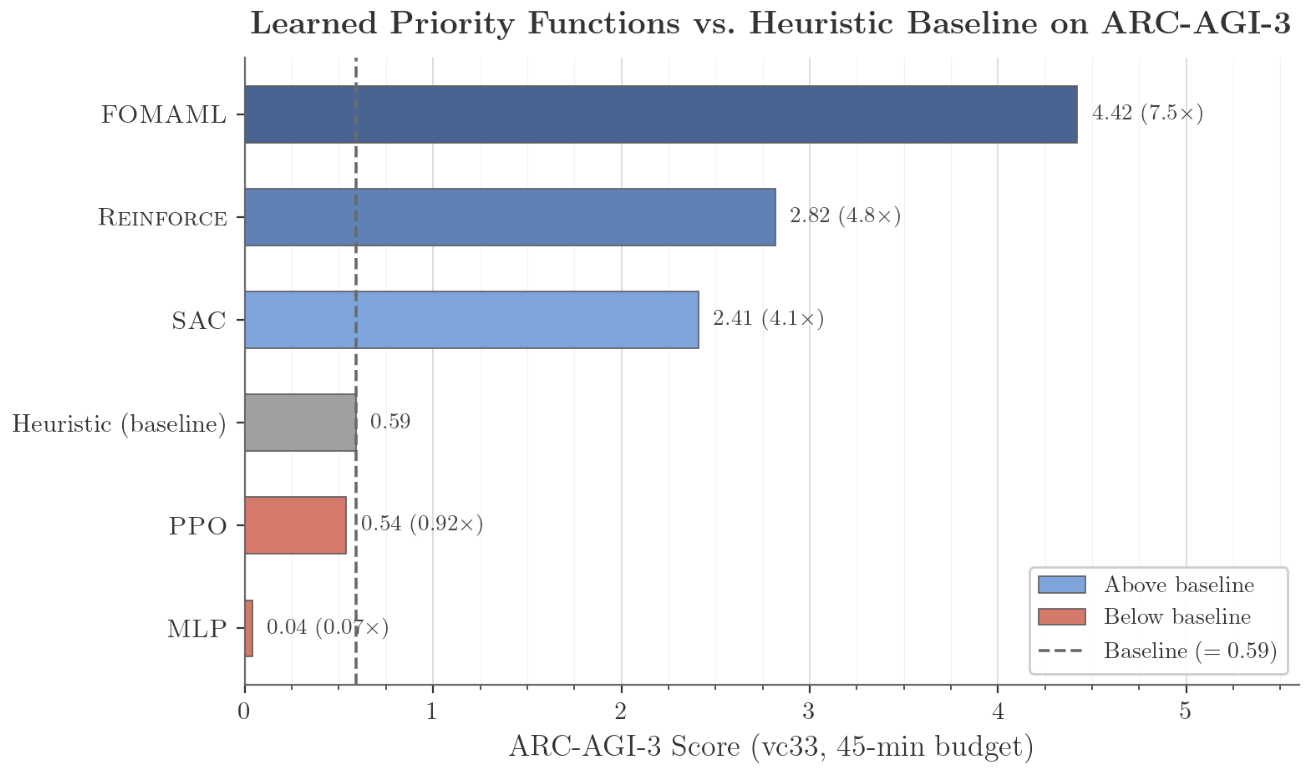
\includegraphics[width=0.95\linewidth]{ModelComps.png}
  \caption{Learned Priority Functions vs. Heuristic Baseline on ARC-AGI-3. Absolute scores and relative performance gains ($x\times$) are evaluated on the \texttt{vc33} clicking game across a 45-minute execution budget.}
  \label{fig:quantitative_results}
\end{figure}
Upon evaluation, FOMAML achieves a score of 4.42, a 7.5× improvement over the heuristic baseline (0.59). REINFORCE reaches 2.82 (4.8×) and SAC reaches 2.41 (4.1×). Both PPO (0.54, 0.92×) and the MLP (0.04, 0.07×) fall below the baseline. Because all agents take approximately the same number of total actions, score differences are driven by how efficiently each agent resolves levels.

\subsection{Qualitative Analysis}

In the vc33 game, levels progressively introduce new interactive elements, so what matters to click at level 1 differs from what matters at level 5. FOMAML's meta-weights are explicitly trained to produce task-weights that adapt quickly at each level boundary. When a new level begins, FOMAML resets its task-weights to the meta-initialization and then takes inner gradient steps, identifying the new level's relevant segments within the first few clicks. REINFORCE, by contrast, accumulates all experience into a single weight vector that must simultaneously balance the optimal priorities for every level it has seen, which is a harder optimization problem.

The warm-started linear model improves on the static heuristic because it receives direct per-click feedback and can revise its beliefs. REINFORCE may discover, for example, that \texttt{closeness\_to\_medium} is a stronger predictor than saturation for this particular game and shift its weights accordingly; the heuristic cannot make this adjustment regardless of how much evidence accumulates against it.

SAC's replay buffer lets it reuse each observed transition across multiple gradient steps, producing more stable Q-estimates than REINFORCE's single-step updates. Its entropy regularization additionally prevents the policy from collapsing onto a small set of high-scoring segments, which matters when later levels require clicking less obvious elements. The modest gap between SAC and REINFORCE suggests that the sample-efficiency benefit of replay is largest early in training, before REINFORCE has accumulated enough signal to stabilize.

PPO requires a full rollout buffer of 32 transitions before any gradient update, so it adapts more slowly than the per-step methods. Because only a fraction of clicks in vc33 produce state transitions, filling the buffer with informative signal takes substantially more wall-clock time than the buffer size alone implies, delaying the policy improvement that clipping and GAE are designed to stabilize.

The MLP's near-zero score (0.04) confirms that random initialization leads to poor priority assignments from the first step, and early gradient updates that overfit to level-1 segments actively harm performance on later levels. Richer model capacity does not compensate for a weak starting point when the data budget is this tight, confirming that the warm start is load-bearing for online RL in this environment.

% \subsection{Quantitative Evaluation}
% \lipsum[26-28]

% \begin{table}
%   \caption{Performance Comparison}
%   \label{tab:performance}
%   \centering
%   \begin{tabular}{lccc}
%     \toprule
%     Method & Metric 1 & Metric 2 & Metric 3 \\
%     \midrule
%     Baseline & 0.75 & 0.62 & 0.81 \\
%     Our Approach & 0.83 & 0.71 & 0.87 \\
%     Variant A & 0.79 & 0.68 & 0.84 \\
%     Variant B & 0.81 & 0.70 & 0.86 \\
%     \bottomrule
%   \end{tabular}
% \end{table}

% \subsection{Qualitative Analysis}
% \lipsum[29-31]

% \begin{figure}
%   \centering
%   % Uncomment and replace with your figure
%   %\includegraphics[width=0.8\linewidth]{results_figure.png}
%   \fbox{\rule{0pt}{5cm}\rule{10cm}{0pt}}
%   \caption{Visualization of results.}
%   \label{fig:results}
% \end{figure}

\section{Discussion}
\emph{FOMAML $>$ REINFORCE $>$ SAC $\gg$ PPO $>$ MLP.}

The above ranking reflects how quickly each agent produces a competent policy in a 45-minute window. FOMAML is fastest because its objective directly optimizes for rapid per-level adaptation. REINFORCE and SAC are fast because their per-step updates require no rollout accumulation. PPO and the MLP are slow because they either defer updates (PPO's rollout buffer) or start from an uninformed initialization (the MLP).

This ordering suggests that the dominant challenge in vc33 is adapting to each level's specific interactive elements within a small number of clicks. ARC-AGI-3 is explicitly designed to reward this kind of fast hypothesis revision through its scoring metric penalizing wasted actions. FOMAML's inductive bias toward rapid local adaptation helped win in this structure.

A secondary finding is that the reward signal we use, a $\pm 1$ binary value issued after every click, is sufficient for online policy improvement despite the fact that most clicks do not produce transitions. In vc33, transition-producing clicks are the informative minority, meaning positive rewards are infrequent. The reward signal is nonetheless dense in the sense that every action generates an observation, and negative signal (this segment type is not interactive at this level) is itself highly informative. This stands in contrast to level-completion reward, which would provide no gradient signal at all for the many levels that no agent completes within the time budget.

The warm-start ablation (comparing the MLP to REINFORCE) isolates the contribution of initialization from the contribution of model capacity. REINFORCE, a linear model, outperforms the MLP by more than 70$\times$. Since the only structural difference is initialization, this result is strong evidence that a competent starting point matters more than expressive capacity in low-data online RL. Practitioners extending this work to richer game environments should prioritize warm-starting from a reliable hand-coded prior.

Several limitations bound these conclusions. First, we evaluate only on vc33, and whether the level-adaptation hypothesis generalizes to other ARC-AGI-3 games with different transition structures is unknown. Second, the 45-minute budget may systematically favor fast-adapting methods, since under a longer horizon PPO and the MLP might eventually exceed REINFORCE once they accumulate sufficient data. Third, our feature set, though an improvement over the binary baseline, is still hand-designed, and a learned visual encoder might surface interactive cues that our four features miss.

\section{Conclusion}
We asked whether replacing a hand-coded visual salience heuristic with a learned priority function improves exploration efficiency in ARC-AGI-3. The answer is yes, with quite a significant improvement. FOMAML achieves a 7.5$\times$ improvement over the baseline, REINFORCE a 4.8$\times$ improvement, and SAC a 4.1$\times$ improvement, all without modifying the underlying graph explorer.

ARC-AGI-3's progressive level structure creates a sequence of distribution shifts, each introducing interactive elements the agent has not seen before. An agent that can identify the new level's relevant segments within its first few clicks accumulates significantly more score than one that slowly converges on a global optimum. FOMAML's explicit optimization for fast adaptation is well-matched to this structure. REINFORCE's simpler per-step updates are sufficient to beat the static heuristic but not to match FOMAML's level-boundary agility.

Future work should evaluate these agents on additional ARC-AGI-3 games to test the generality of the level-adaptation hypothesis and investigate whether a learned visual encoder can replace the hand-designed feature set.
\section{Team Contributions}
\begin{itemize}
  \item \textbf{Ryan Bookman:} Developed the core online policy optimization infrastructure. Programmed the algorithmic architectures for the baseline REINFORCE model, the non-linear Neural Network, and the meta-learning First-Order MAML frameworks.
  \item \textbf{Steve Mendeleev:} Engineered the robust multi-threaded parallel execution infrastructure and evaluation pipeline. Programmed the PPO agent wrapper, designed the unified telemetry logger, and managed the end-to-end benchmarking runs on the central API server.
  \item \textbf{Kyle Feinstein:} Headed the off-policy sample-efficiency research track. Implemented the Soft Actor-Critic architecture, constructed its experience replay buffer mechanics, and tuned the automated online entropy regularization system.
  \item \textbf{All Authors:} Collaborated on the initial feature engineering design space, established the mathematical formulations for the continuous closeness-to-medium metric, and co-developed the algorithmic integration strategy linking the learned scoring layers to the upstream graph explorer.
\end{itemize}

\paragraph{Changes from Proposal} We originally proposed RL replacing uniform random action selection in exploration. Instead, we apply RL to learn the priority group assignments themselves.

\bibliographystyle{ACM-Reference-Format}
\bibliography{reference}


% ============================================================================
% APPENDIX
% ============================================================================
\appendix

% \section{Additional Experiments}
% \lipsum[19]

% \section{Implementation Details}
% \lipsum[20]

\section{AI Use Disclosure}
We used Claude to assist with refining our wording in the paper and also to catch some bugs in our code. Claude also helped us with some unrelated boilerplate infrastructure (logging setup, threading, test scaffolding). The core project design, experiments, and analysis were completed independently by the team.

\end{document}